\documentclass{article}\usepackage[]{graphicx}\usepackage[]{color}
% maxwidth is the original width if it is less than linewidth
% otherwise use linewidth (to make sure the graphics do not exceed the margin)
\makeatletter
\def\maxwidth{ %
  \ifdim\Gin@nat@width>\linewidth
    \linewidth
  \else
    \Gin@nat@width
  \fi
}
\makeatother

\definecolor{fgcolor}{rgb}{0.345, 0.345, 0.345}
\newcommand{\hlnum}[1]{\textcolor[rgb]{0.686,0.059,0.569}{#1}}%
\newcommand{\hlstr}[1]{\textcolor[rgb]{0.192,0.494,0.8}{#1}}%
\newcommand{\hlcom}[1]{\textcolor[rgb]{0.678,0.584,0.686}{\textit{#1}}}%
\newcommand{\hlopt}[1]{\textcolor[rgb]{0,0,0}{#1}}%
\newcommand{\hlstd}[1]{\textcolor[rgb]{0.345,0.345,0.345}{#1}}%
\newcommand{\hlkwa}[1]{\textcolor[rgb]{0.161,0.373,0.58}{\textbf{#1}}}%
\newcommand{\hlkwb}[1]{\textcolor[rgb]{0.69,0.353,0.396}{#1}}%
\newcommand{\hlkwc}[1]{\textcolor[rgb]{0.333,0.667,0.333}{#1}}%
\newcommand{\hlkwd}[1]{\textcolor[rgb]{0.737,0.353,0.396}{\textbf{#1}}}%
\let\hlipl\hlkwb

\usepackage{framed}
\makeatletter
\newenvironment{kframe}{%
 \def\at@end@of@kframe{}%
 \ifinner\ifhmode%
  \def\at@end@of@kframe{\end{minipage}}%
  \begin{minipage}{\columnwidth}%
 \fi\fi%
 \def\FrameCommand##1{\hskip\@totalleftmargin \hskip-\fboxsep
 \colorbox{shadecolor}{##1}\hskip-\fboxsep
     % There is no \\@totalrightmargin, so:
     \hskip-\linewidth \hskip-\@totalleftmargin \hskip\columnwidth}%
 \MakeFramed {\advance\hsize-\width
   \@totalleftmargin\z@ \linewidth\hsize
   \@setminipage}}%
 {\par\unskip\endMakeFramed%
 \at@end@of@kframe}
\makeatother

\definecolor{shadecolor}{rgb}{.97, .97, .97}
\definecolor{messagecolor}{rgb}{0, 0, 0}
\definecolor{warningcolor}{rgb}{1, 0, 1}
\definecolor{errorcolor}{rgb}{1, 0, 0}
\newenvironment{knitrout}{}{} % an empty environment to be redefined in TeX

\usepackage{alltt}
\title{Germination phenology as a seasonal priority effect; competition between native \textit {Cryptotaenia canadensis} and invasive \textit{Hesperis matronalis} seedlings is mediated by their relative timing of germination in pair-wise competition trials.}
\IfFileExists{upquote.sty}{\usepackage{upquote}}{}
\begin{document}
\maketitle
\section{Introduction}
\textbf{A core task of invasion biology it to identify trait that make a species likely do be invasive}
\begin{enumerate}
\item Invasive species are characterized by rapid germination and precocious phenology
\item Being so early may function as a seasonal priority effect-niche premption and such
\item This seasonal priority effect might contribute to the competitive dominacne and invasion success of invasives
\end{enumerate}

\textbf{But it is difficult to infer mechanism from observational studies}
\begin{enumerate}
\item Because rapid phenology often covaries with other competitive traits. You'd need super high resolution phenolgy and climate data.
\end{enumerate}

\textbf{Experiments can test role of SPE's in plant competition}
\begin{enumerate}
\item  A common approach is to use sequential planting studies.
\item recent review paper on these experiments by \citet{Weidlich:2020aa}: 42\% of such studies included planting interval treatments of less than 1 month, approximating the time scale of SPEs and all found evidence of priority effects. (How many were invasive vs. native?)
\end{enumerate}

\textbf{Yet the extent to which these studies are generailizable is questionable}
\begin{enumerate}
\item  Almost all mechanistic tests for SPEs to date have been performed using species from temperate grasslands \citep{Weidlich:2020aa}, whose germination behavior may differ substantially from taxa in other habitats \citep{Tudela-Isanta:2018aa}.
\item In many ecosystems, plant communities must re-assemble each year after a period of dormancy. In these communities, priority effects are largely the product of the rate at which dormant plants and seeds respond to their environment and resume growth or germinate when favorable conditions return \citep{Rudolf:2019aa}, rather than the the timing of the arrival of propagules, which in many cases occurs prior to the dormant season \citep{Howe:1982aa,Baskin:1988aa}.
\item Therefore, sequential plantings cannot address how important SPE's are in nature because the priority effect is 100\% contigent on the choice of the treatment.
\end{enumerate}

\textbf{In ecological systems where dormancy is common like temperate  and boreal forest, say a few other here, environmental conditions such as temperature (cold stratification and incubate), soil moisture, and light control the release of dormancy and germination or growth.}
\begin{enumerate}
\item Cohabiting species respond with different sensitivites to these elements; and this may be especially true for invasive species which evolved under different climate condition in their home vs. invaded ranges.
\item And climate elements vary over time
\item Together, this suggests that germination or phenological responses between competing species will converge and divirge periodically over time, depending the their specific sensitives and the climate they experience.
\item This variation can be leverage for mechanistic tests of SPEs by a) qunatify how the phenoligical lag between species changes under realistic climate variation , and b) the effect of this variation on competition
\end{enumerate}

\textbf{Leveraging natural climate variation to test SPEs has major beneifits}
\begin{enumerate}
\item SPE's are a cornerstone of community assembly theory and modern coexistence theory, and mechansitically qunatifying their contribtion in community interactions is important
\item Anthropogenic climatic change is altering the  environments \citep{Walck2011} and changing  germination and phenology patterns. Such sustained alterations to environmental cues have potential to disrupt SPEs, shifting balances of species' interactions, changing patterns of invasion, and strongly influence biological filtering of communities..
\item So assessing the role of SPE's in species interactions under more realistic germination environments is timely because it can be used to improve spatio-temporal predictions of species interaction under novel climate conditions.
\end{enumerate}

\textbf{While invasibility, competion, coexistance etc is a property of individual and community interactions, pair-wise comparisons have been a useful tool to identifying and quatify mechanisms of species interactions}
\begin{enumerate}
\item Why am I saying this? Probably to justify the limited taxonomic scope of my study
\end{enumerate}

\textbf{Using a combination of germination assays, competition trials and climate projections, we:}
\begin{enumerate}
\item Quantify gernmination behavior of varying environments to estimate a realistic range of climate driven priority between an widespread invasive and native forb species. 
\item Compete them to assess the influences of priority effect on competitive outcome and quantify SPE's contribution vs. other intrinsic competition traits.
\item Use relationship between climate and germination behavior to make first-pass, quick and dirtay and rough prediction about where where interactions between these two species may shift with climate change as a proof-of-concept case study to build on in the future.
\end{enumerate}

\section*{Methods}
\subsection*{Focal species}
\subsection*{Germination Assays}
\subsection*{Competition Trials}
\subsection*{Data analysis}
\textbf{Some thoughts on Connolleys RGRD models}
\begin{enumerate}
\item Data at the plot level which makes large assays like the one I did tractable compared with spatially explict ones like heygi index or neighborhood
\item Also is desinged for signle season dynamics unlike Lotke-Volterra and the usual
\item Weakness, isn't designed for monoculture treatments( which we explictely put in out study ) since you an't have the log of zero. Maybe I overcome this by converting 0s to 00000.1

\end{enumerate}


\section*{Discussion}
\textbf{So many caveats:}
\begin{enumerate}
\item These species are perennials, seeds banks. Given our expermental constrait couldn't account for these dynamics. ie competition my happen between raments and seeds. Our simplifed experimental design doesn't address these important factors, however they add an important piece to the puzzle. 
\item Given above, our results may be most relevant in colonization dynamics, especially in super disturbed systems where seed ins important.
\item Limitations of RGRD models from paper
\item We know invasives invade communities not population, two species studies are limited to predict the invasion dynamics of a species in real time
\item What we did do was quantify the contribution of priority effect to invasion success. It's high. This suggest restorations could benefit from consider phenological diversity 
\end{enumerate}

\begin{figure}[h!]
    \centering
         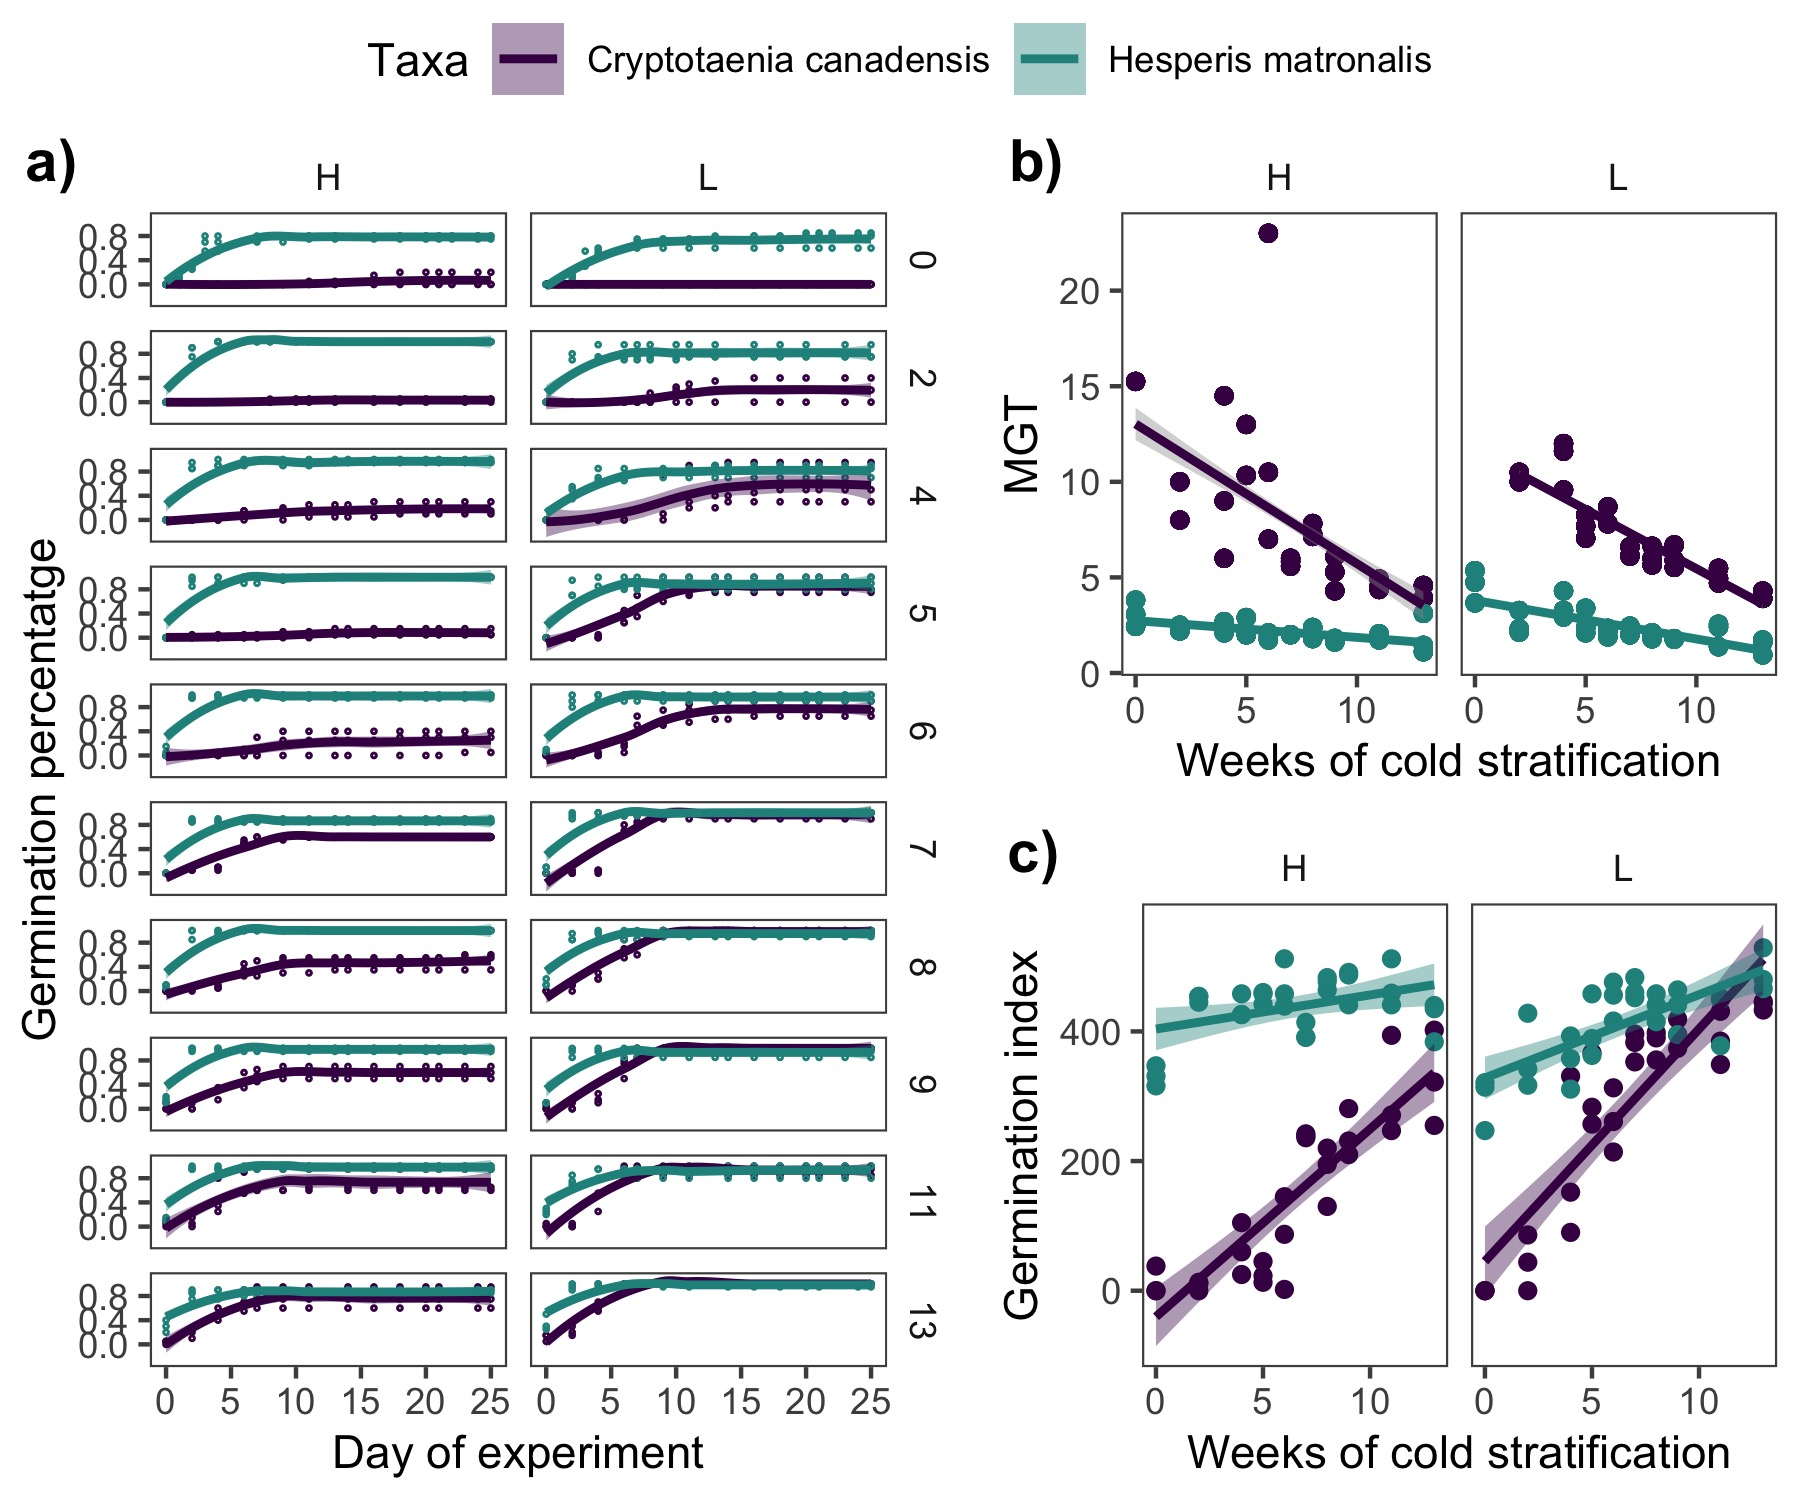
\includegraphics[width=\textwidth]{..//figure/crp_hesp1.jpeg}
    \caption{Germination behavior of \textit{H. matronalis} and \texit{C. canadensis} indicate that the rate of \texit{C. canadensis} approaches that of \textit{H. matronalis} under cool temperatures and high levels of stratification. a) Shows germination time courses for both species at each level of incubation (H,L) and stratitification (0-13, y-axis). b) Dipicts Mean germination time for each species as a function of weeks of stratifcation and both high (H) and low (L) incubation temperature. c) Show a composite germination index for each species that account for the speed and percentage of germination for each species as a function of weeks of stratifcation and both high (H) and low (L) incubation temperature. } 
    \label{fig:aft}
\end{figure}

\begin{figure}[h!]
    \centering
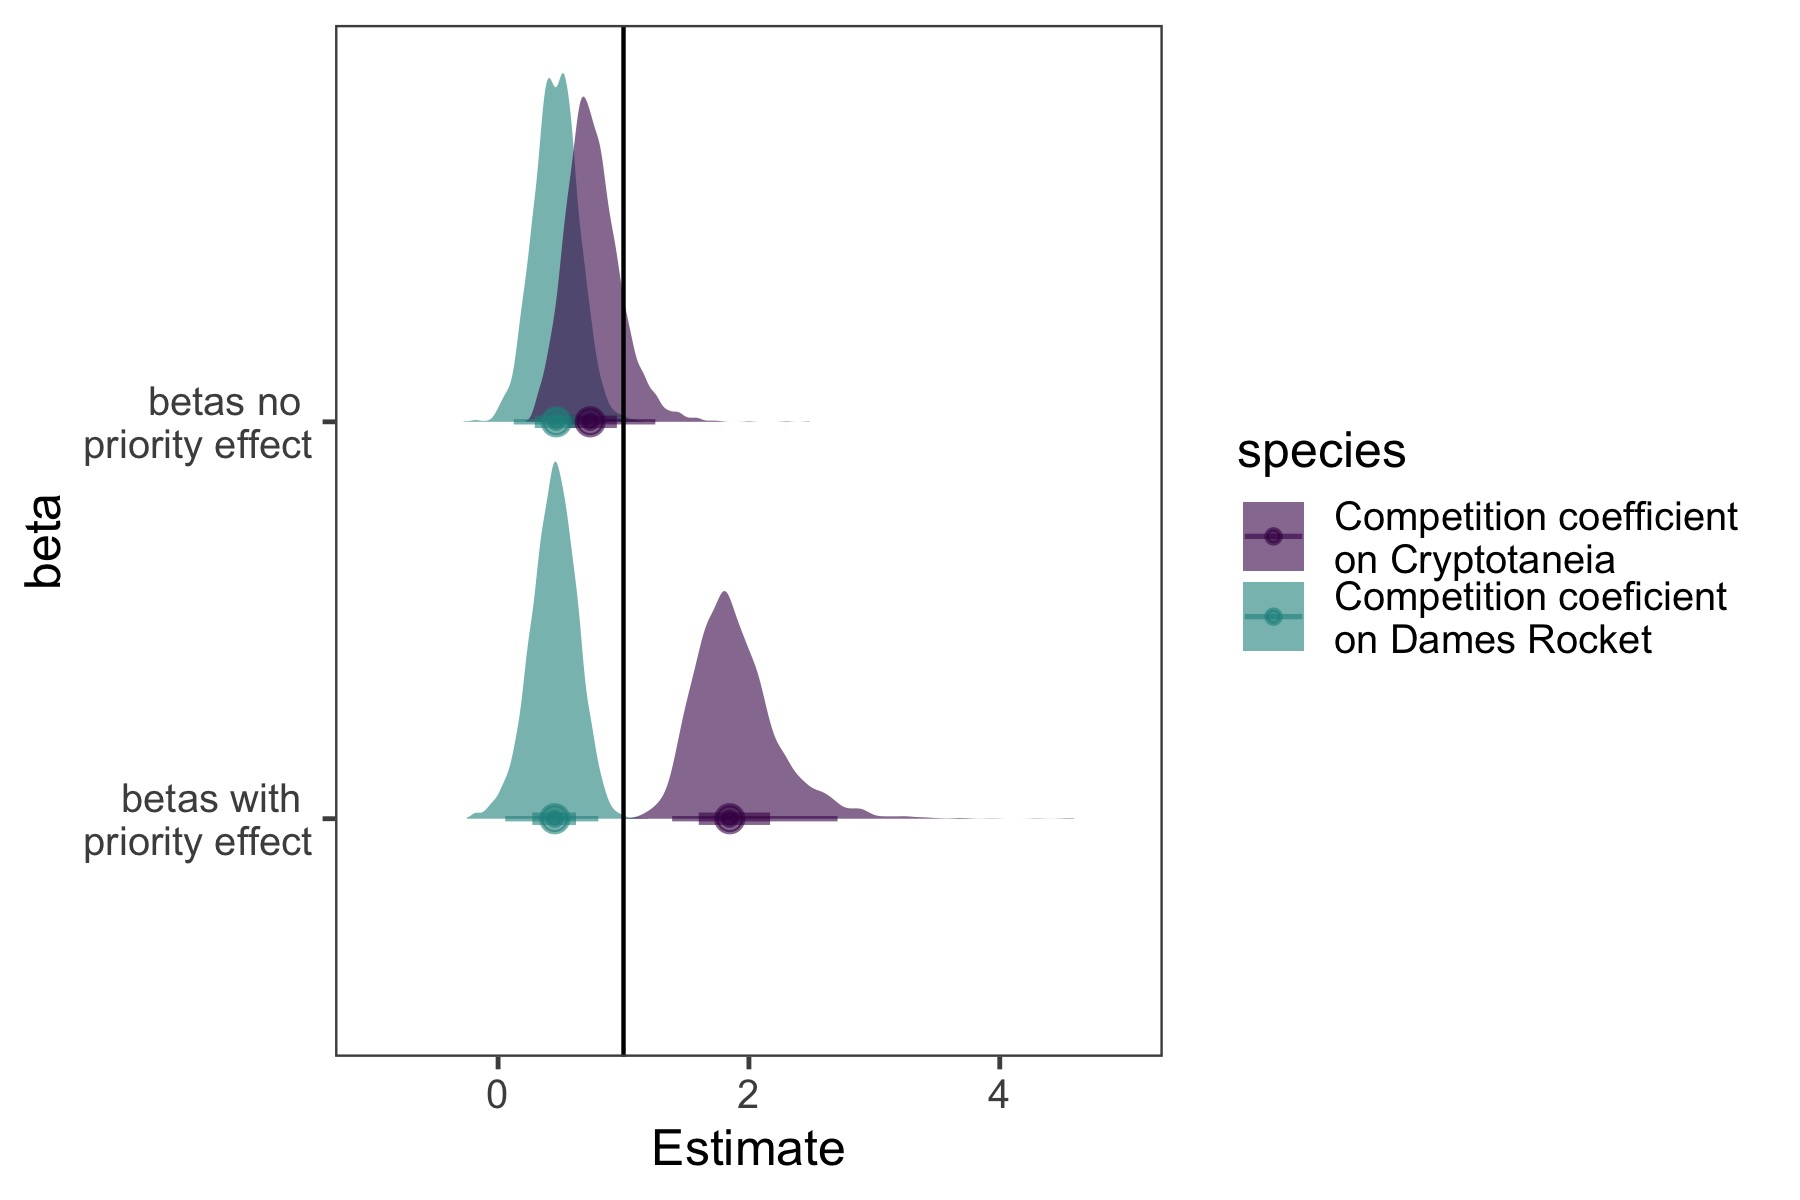
\includegraphics[width=\textwidth]{..//figure/comp_coefficient.jpeg}
    \caption{Estimated of competition coefficients with and without priority effect. Without priority effect, species would be expected to coexist (for both species, intra-specific competition is highe than interspecific i.e. coefficients are less than one). When just one day of priority effects are included in the calculation Dames rocket's interspecific competition increases realtive to its intraspecific competition strength, suggesting with will ultimately competitively exclude Honewort.  } 
    \label{fig:Cc}
\end{figure}

\begin{figure}[h!]
    \centering
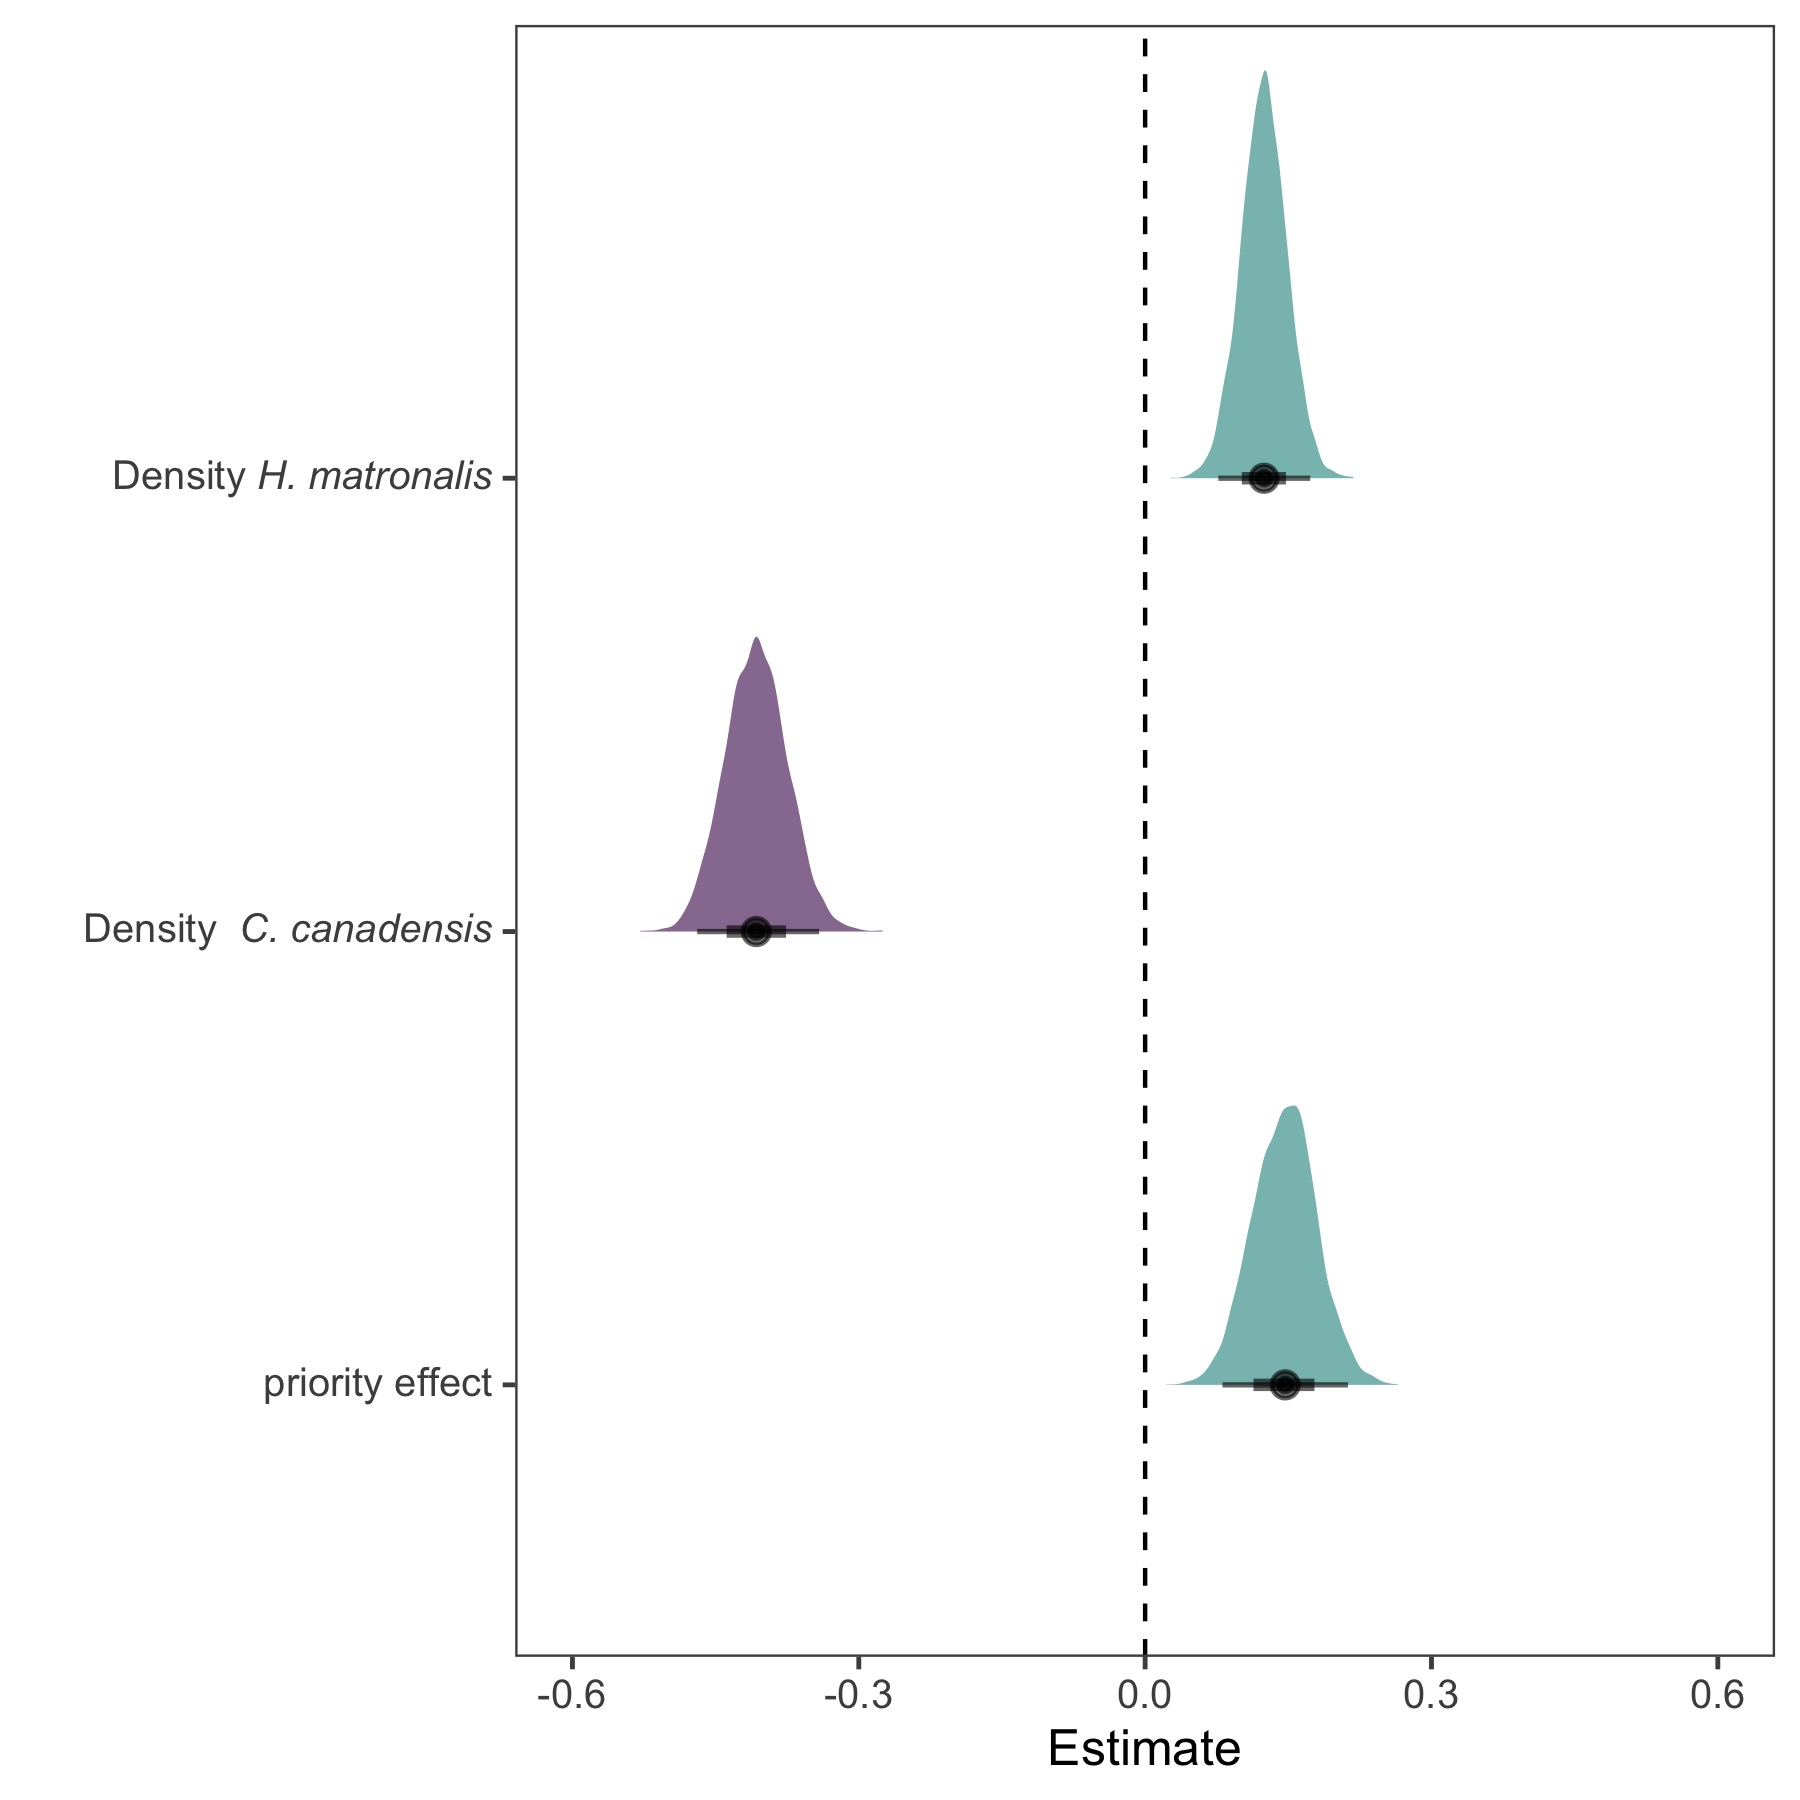
\includegraphics[width=\textwidth]{..//figure/mu_plots.jpeg}
    \caption{Estimated effects of density influence parameters and temporal priority effect on the relative growth rate difference between \textit{H. matronalis} and \texit{C. canadensis}. As per Connonly and Wayne 2005, The positive estimate of priorty and density of Hesperis matronalis tip competitive balance towards it, while the negative estimate of density of C. canadensis favor that species. Like Fig. 2, this suggests that priorty effects are a key mediator of competitive sucess in H. matronalis.  } 
    \label{fig:Cc}
\end{figure}

\begin{figure}[h!]
    \centering
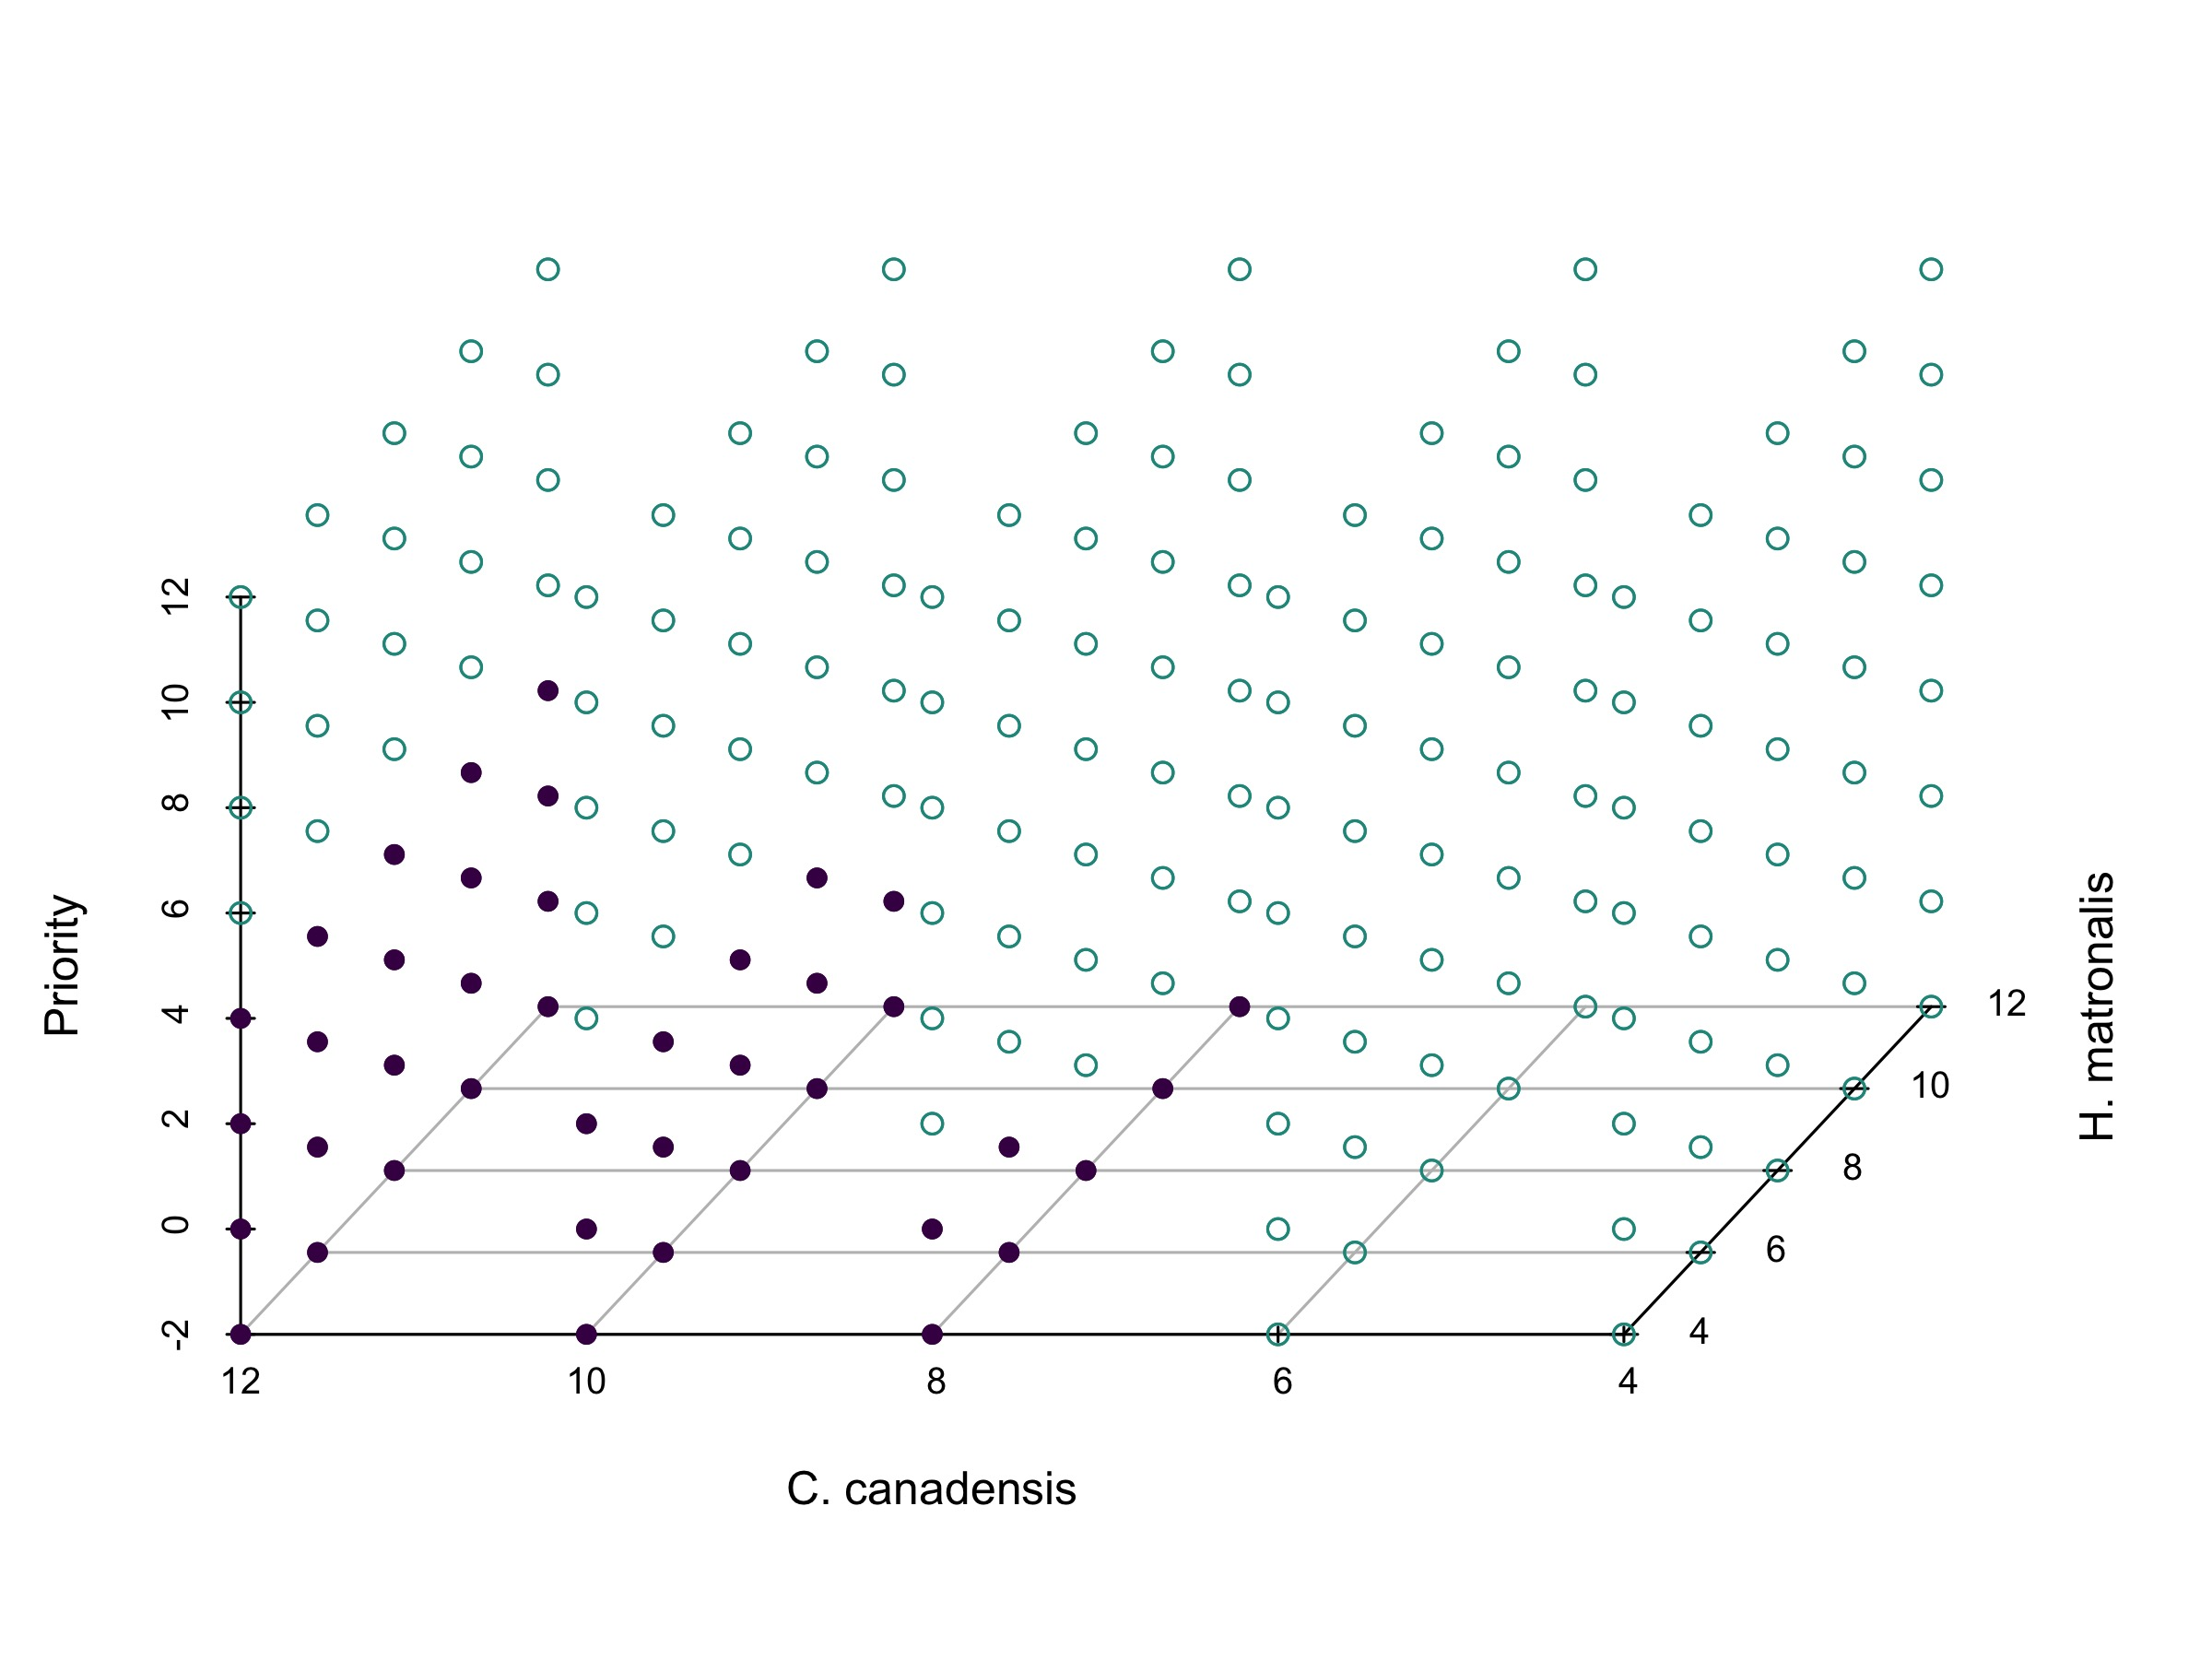
\includegraphics[width=\textwidth]{..//figure/threedpred.jpeg}
    \caption{Predicted outcome of competition under vary inter-specific densities and temporal priority. Purple is \texit{C. canadensis} and green \textit{H. matronalis}. Need to add legend here. As can been seen C. canadensis is predicted to compete with H matronalis only at low priority effects or high densities. } 
    \label{fig:Hm}
\end{figure}





\end{document}
